\begin{frame}[allowframebreaks]{General-Attention Vs Self-Attention}
    \begin{figure}
        \flushleft
        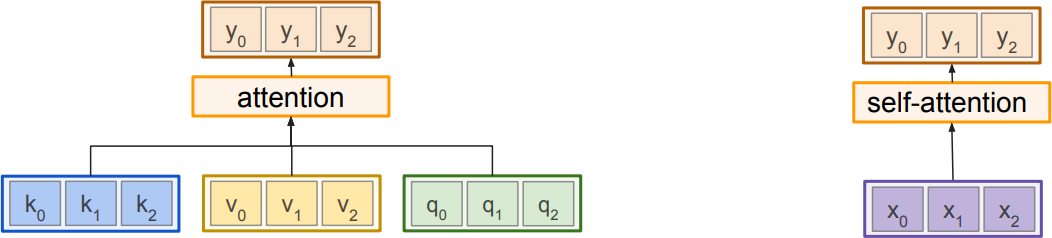
\includegraphics[width=\linewidth,height=\textheight,keepaspectratio]{images/transformers/slide_48_1_img.png}
    \end{figure}
    \vspace{0.5cm}
    \begin{table}[ht]
        \centering
        \begin{tabular}{|l|p{3.5cm}|p{3.5cm}|}
            \hline
            \textbf{Comparison} & \textbf{General Attention} & \textbf{Self-Attention} \\
            \hline
            Q, K, V origins & From separate source \& target & From same input sequence \\
            \hline
            Use case & Encoder $\rightarrow$ Decoder cross-attention & Encoder/Decoder internal relation info \\
            \hline
            Information flow & Across representations & Within single representation \\
            \hline
        \end{tabular}
        \caption{General Attention vs. Self-Attention}
    \end{table}
\end{frame}